\hspace{0.5 cm}
Pentru a putea interpreta datele rezultate le-am clasificat manual într-un tabel, precum cel din cadrul competiției pentru a putea face o comparație între ele. Câmpurile de tabel sunt următoarele:
\begin{itemize}
    \item \textbf{Benchmark}: Benchmark-ul pentru care avem înregistrate rezultatele.
    \item \textbf{neural network (ONNX)}: Fișierul ONNX pentru care a rulat tool-ul.
    \item \textbf{specifications (VNNLIB)}: Fișierul VNNLIB pentru care a rulat tool-ul.
    \item \textbf{results (vnncomp2023/us)}: Poate avea valori sat/unsat; sat înseamnă că modelul îndeplinește condițiile din fișierul VNNLIB, adică distanța aproximată de discriminator este aceeași cu distanța pe care a primit-o generatorul ca și dată de intrare; unsat înseamnă că discriminatorul nu a reușit să facă o aproximare corectă.
    Prima coloană cu rezultate reprezintă rezultatele obținute în competiție, iar a două coloană cu rezultate este obținută de noi.
    \item \textbf{time to verify (vnncomp2023/us)}: Timpul de rulare a tool-ului pentru o instanta. Prima coloană reprezintă timpii obținuți în competiție, iar cea de-a doua coloană reprezintă timpii obținuți de noi.
\end{itemize}

În tabelul din figura \ref{fig:image1}, se prezintă o analiză comparativă între rezultatele obținute în urma rulării proprii și cele obținute în cadrul competiției.

\begin{figure}[h]
\centering 
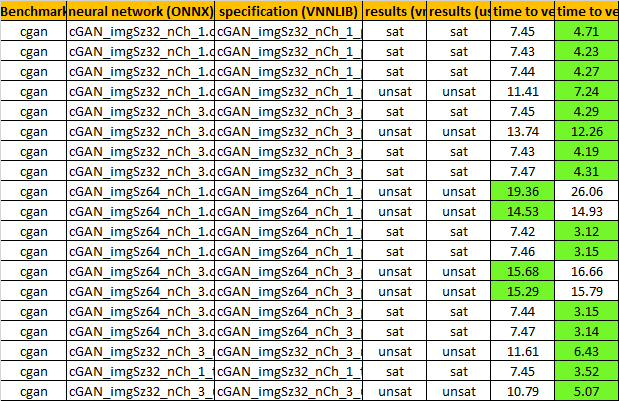
\includegraphics[width=0.8\linewidth]{imagini/interpretare rezultate/abC_comp_vs_us.png}
\caption{Comparare rezultate alpha-beta-CROWN}
\label{fig:image1} 
\end{figure}
\

Conform tabelului \ref{fig:image1}, este de remarcat faptul că pentru fiecare intrare, rezultatele (sat/unsat) au fost aceleași, atât pentru rezultatele rulării noastre, cât și pentru cele din competiție. Diferența dintre rezultatele din competitie si cele extrase de echipa noastră o constituie timpul de verificare.
În tabel sunt evidențiați cu culoarea verde timpii mai reduși de verificare pentru aceleași instanțe.

Timpul de verificare înregistrat al echipei este în medie mai mic cu aproximativ 3 secunde pentru intrările unde rezultatul este satisfiabil. În schimb, pentru intrările cu rezultat nesatisfiabil am obtinut un timp de verificare mai mare comparativ cu cel din competitie.

Graficul \ref{fig:image3}, evidențiază și mai mult distribuirea timpilor de execuție pentru fiecare instanță în parte.

\begin{figure}[h]
\centering 
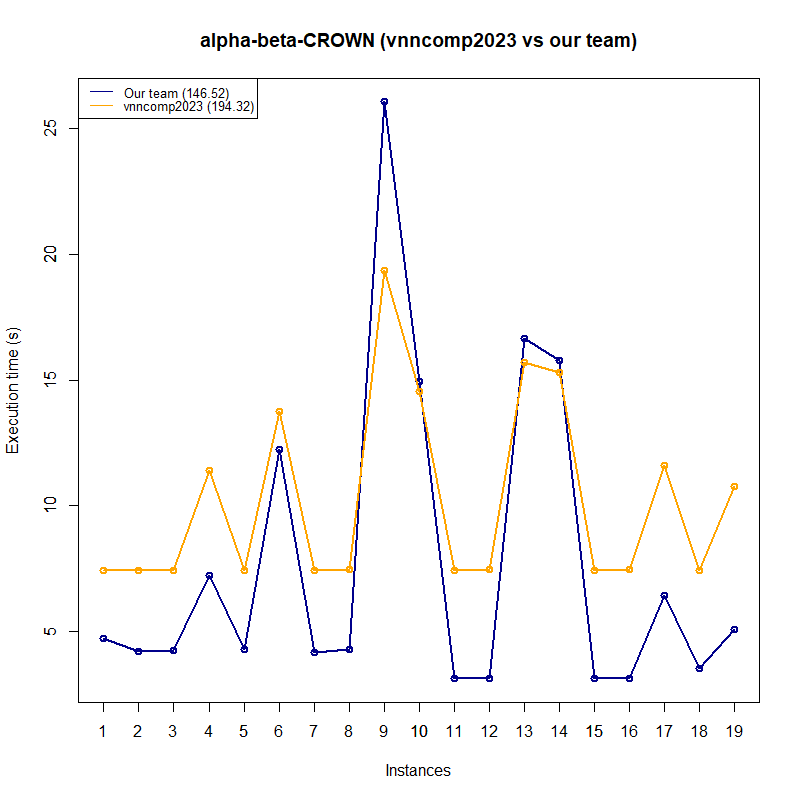
\includegraphics[width=0.8\linewidth]{imagini/interpretare rezultate/abC_us_vs_vnncomp.png}
\caption{Comparare rezultate alpha-beta-CROWN}
\label{fig:image3} 
\end{figure}
\